
This document describes the ``reload'' of the H$\to$WW$\to2l2\nu$
analysis for the Lepton Photon 2011 conference.  The reload primarily
adds extra data to the existing analysis, but also includes minor
technical changes such as the residual energy scale correction, Monte
Carlo re-weighting for new pile-up conditions and a new luminosity
estimation.

The final dataset (LP) used for the analysis corresponds to \lpintlumi~
of data. For comparison with the EPS conference results we split the
data sample in two parts: EPS (\intlumi) and post-EPS (0.4 fb$^{-1}$).

To update the analysis we first validated the post-EPS data. We find
the post-EPS data to be consistent with the EPS data with regard to
trigger and lepton efficiencies
(Tables~\ref{tab:lp_eff_electrons}-\ref{tab:lp_eff_muons}). Because we
do not observe any significant change in the lepton selection
efficiencies, we perform the LP analysis using the same data to
simulation scale factors as the EPS analysis. We find good agreement
between data and MC for the distribution of the number of
reconstructed vertices per event after re-weighting based on the
expected number of pile-up events.  We inspected the relevant
kinematic variables and find no significant discrepancies between the
two data samples (Appendix~\ref{app:lp_postEPSdist}).

We then performed the background estimations. The rate for each
background process is found to be stable in the EPS, post-EPS and full
LP data
samples. Tables~\ref{tab:routin_lp_data_0j}-\ref{tab:lp_periods_ww}
summarize the results for all dominant backgrounds. Observed
background yields per unit of luminosity are consistent for EPS
and post-EPS data. In the light of recent discussions of the
W$\gamma^{(*)}$ background, it is worth to point out that the closure
test on same-sign events gives good agreement with the expectations,
as shown in Table~\ref{tab:lp_FakeLeptonBkgPrediction_SameSignSample}.

The observed and expected upper limits correspoinding to full LP data
set are shown in Figure~\ref{fig:limits_final}.

\begin{figure}[!htbp]
\centering
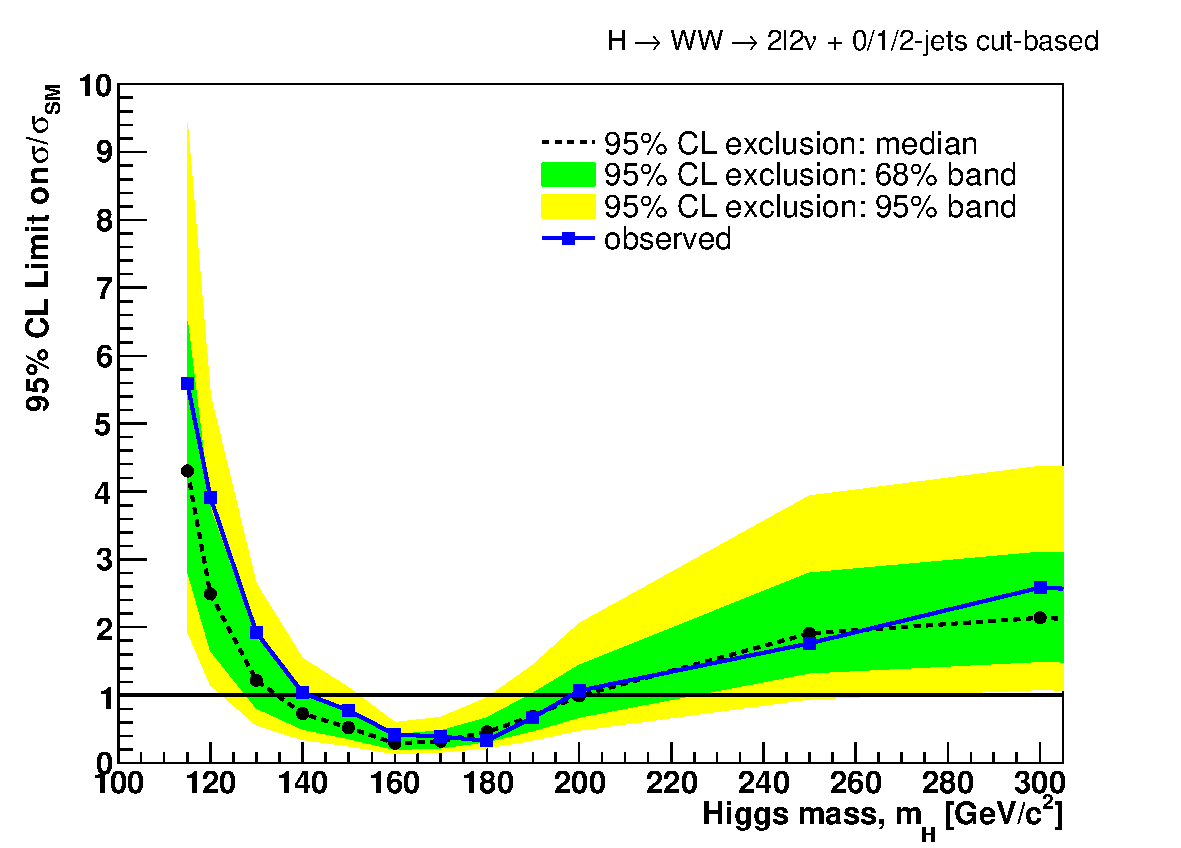
\includegraphics[width=0.48\textwidth]{lp_figures/limits_nj_cut_ana_v6_1500pb_LP.pdf}
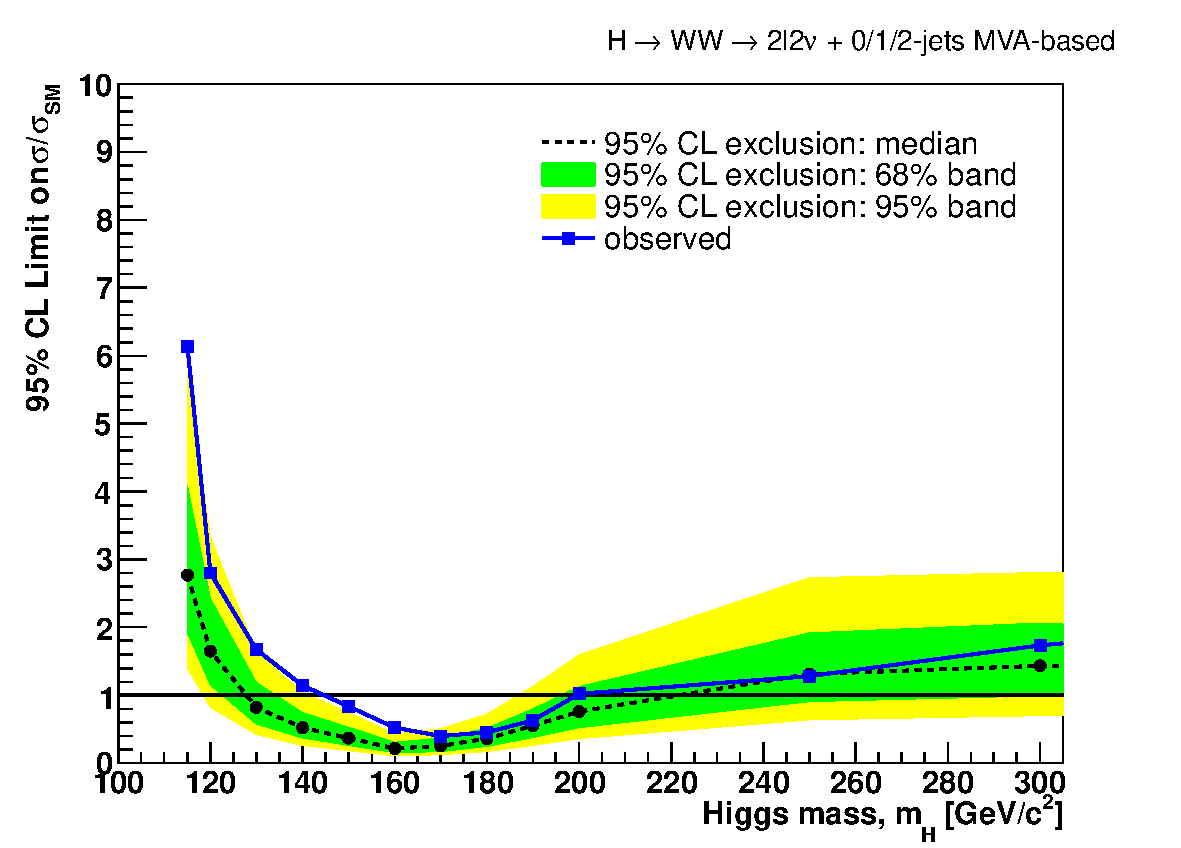
\includegraphics[width=0.48\textwidth]{lp_figures/limits_nj_shape_ana_v6_1500pb_LP.pdf}
\caption{Cut-based analysis (left) and multivariate-based analysis (right) upper limits at 95\% C.L. using data corresponding to 1.5~$\ifb$.
}
\label{fig:limits_final}
\end{figure}

In order to better understand the results we compared upper limit
results for EPS, post-EPS and full LP datasets in
Figures~\ref{fig:limits_0j_cut}-\ref{fig:limits_1j_shape}.

We notice that overall the post-EPS data show much better agreement
between observed and expected limits. In 0-jet case for same-flavor
events we see a downward fluctuation in both cut based and mva based
analyses (Figure~\ref{subfig:post_0j_sf_cut} and
\ref{subfig:post_0j_sf_shape}). In 1-jet case for same-flavor events
we see the observed limits to be consistent with the expected limits
(Figure~\ref{subfig:post_1j_sf_cut} and \ref{subfig:post_1j_sf_shape}
in both cut based and shape based analyses. It is different from the
EPS result (Figure~\ref{subfig:eps_1j_sf_cut} and
\ref{subfig:eps_1j_sf_shape}) that showed around 2$\sigma$ deviation
from the expected limits. This observation supports the idea that the
excess in 1-jet same-flavor events is likely to be just a fluctuation
and suggests that Drell-Yan background is under control.

%
%
%
\subsection{Additional Transverse Mass Selection Requirement}

We propose an additional selection requirement that can
be used to give extra confidence to the analysis. In general, a
requirement that $80 < M_T < m^{Higgs}$ would remove poorly understood
regions with only a negligible reduction in sensitivity.
Specifically, we refer to the following:

\begin{itemize}
    \item There is a concern that $W\gamma^*$ FSR background with
      $W\rightarrow \ell\nu$ and $\gamma^*\rightarrow\ell\ell$ could be
      a significant unaccounted background.  The $M_T$ of the
      reconstructed $e^{+}e^{-}$+MET system should be less than or
      equal to the expected $M_T$ from the decay of a $W$ boson.
    \item The \dytt~background is estimated entirely from simulation.
      This background manifests itself at low $M_T$, as illustrated in
      Figure~\ref{fig:ww_mthiggs_lp}.
    \item Other backgrounds such as W+jets and WW are reduced by
      removing the low $M_T$ region.
\end{itemize}

The yield cross check using same-sign events bounds the $W/\gamma*$ background
at something less than 10 events at WW preselection level.
This bound has the caveat that if the background is large and the
fake rate method understimates the real background then the two
effects can cancel.

The default conversion rejection algorithm used in this analysis
includes a 2 cm flight distance (Lxy) cut, so would not reject this background
from apparently prompt conversions.
Taking into account the expected efficiency of our conversion
rejection algorithm, and removing the Lxy cut,
we would expect to reject $30-50$\% of the residual
$\gamma*\rightarrow e^{+}e^{-}$ background.
Performing this test we remove four events at the WW preselection level.
This reduction in the observed yield is consistent with expectations
from WW, W+jet and W+$\gamma$ simulation.
The events removed are distributed randomly in $M_T$.

Although we do not find evidence of a large unaccounted $W/\gamma*$ background,
we cannot conclusively prove that it is absent either.
We note that the proposed cut would reduce the \dytt~background from an expectation
of around 13 events to below one event in the one-jet bin $e-\mu$ final state at
the MVA preselection level.

\begin{figure}[!htbp]
\centering
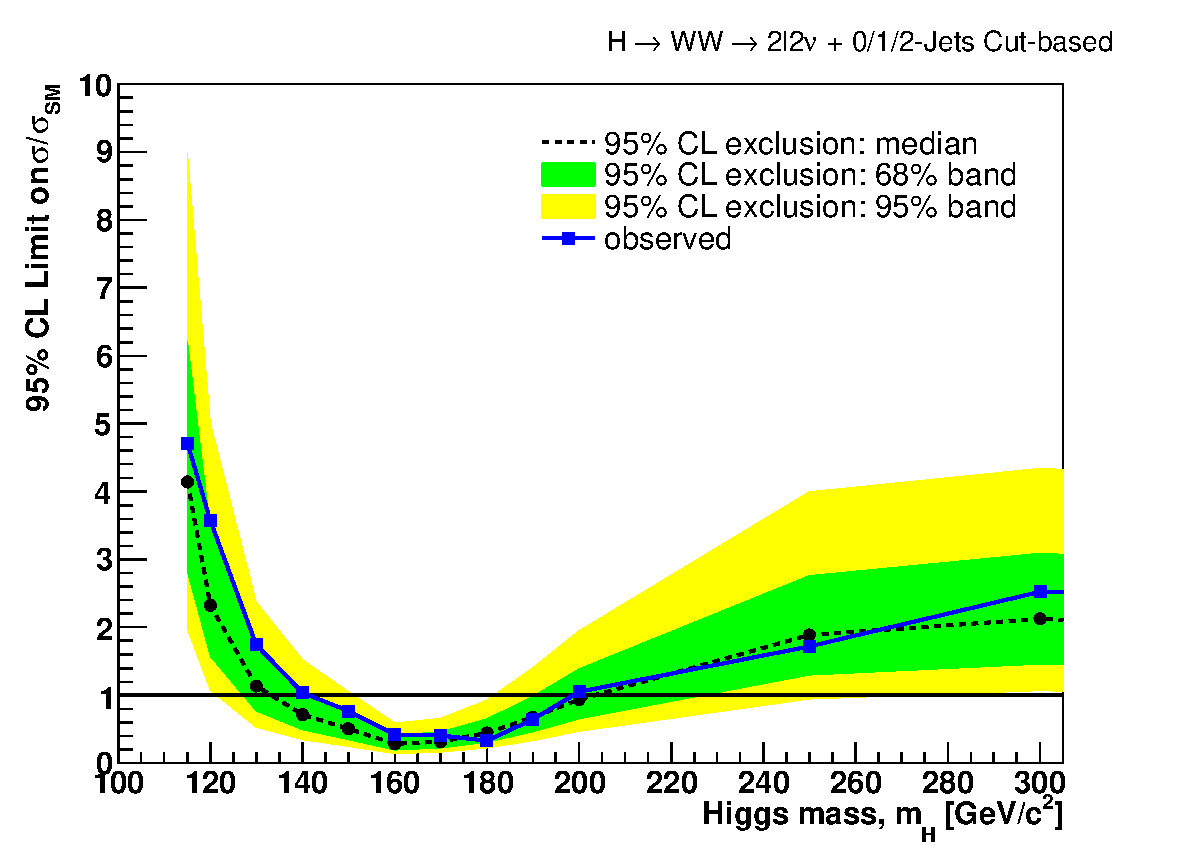
\includegraphics[width=0.48\textwidth]{lp_figures/limits_nj_cut_ana_v6_1500pb_LP_MTCUT80.pdf}
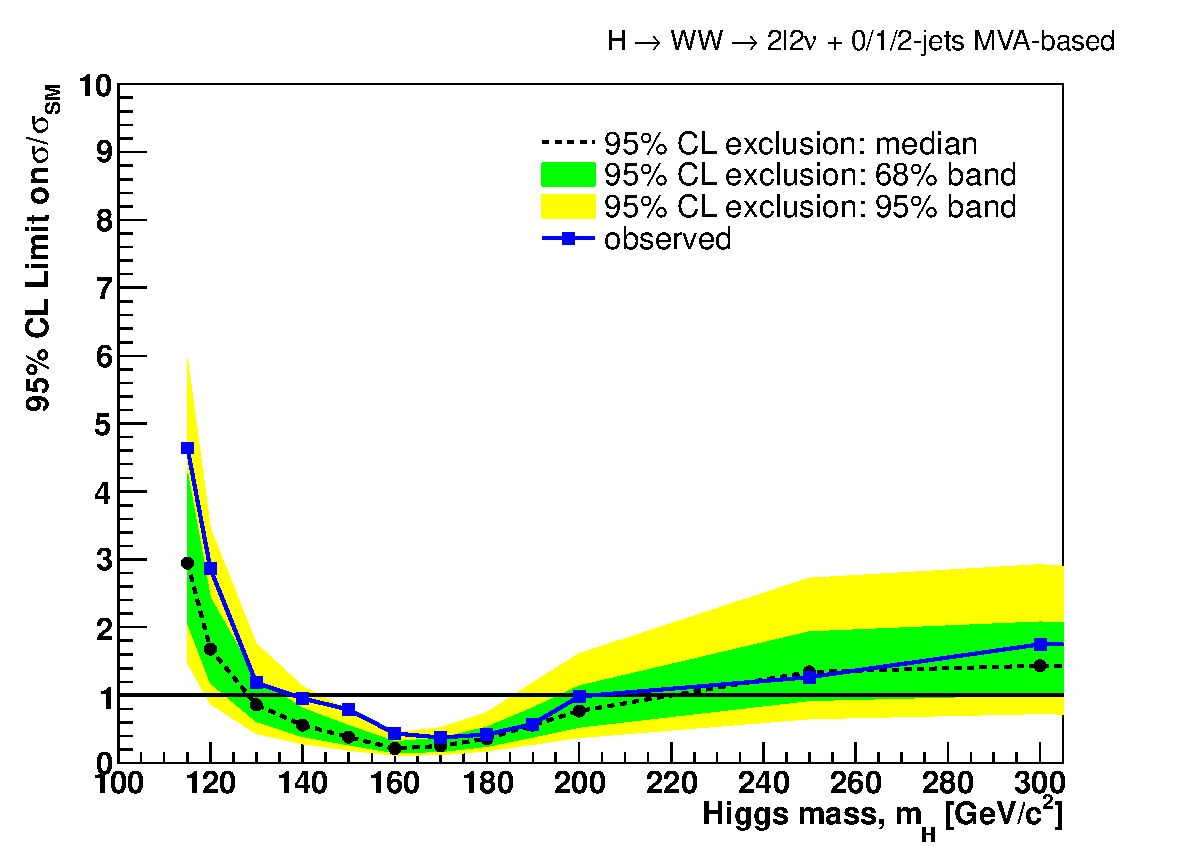
\includegraphics[width=0.48\textwidth]{lp_figures/limits_nj_shape_ana_v6_1500pb_LP_MTCUT80.pdf}
\caption{Cut-based analysis (left) and multivariate-based analysis (right) upper limits at 95\% C.L.
using data corresponding to 1.5~$\ifb$ applying the additional $m_T$ cut.}
\label{fig:limits_final_mt80}
\end{figure}

Figures \ref{fig:limits_final_mt80}, \ref{fig:limits_lp_mtcut80_cut} and
\ref{fig:limits_lp_mtcut80_shape} show results with the $M_T$ cut
applied. It has negligible effect on the expected analysis sensitivity
at all mass points. The observed limits get closer to the expected
ones at low Higgs mass points. This can be either a background
reduction effected or a statistical fluctuation.

